\documentclass[11pt,a4paper]{article}

\usepackage[utf8]{inputenc}
\usepackage[T1]{fontenc}
\usepackage[spanish,es-tabla,es-noshorthands]{babel}
\usepackage{lmodern}
\usepackage[margin=2.2cm]{geometry}
\usepackage{graphicx}
\usepackage{booktabs}
\usepackage{array}
\usepackage{tabularx}
\usepackage{enumitem}
\usepackage[table]{xcolor}
\usepackage{caption}
\usepackage{float}
\usepackage{amssymb}
\usepackage{fancyhdr}
\usepackage[hidelinks]{hyperref}

\definecolor{azul}{HTML}{1C5CAB}
\definecolor{azulclaro}{HTML}{E8F0FB}
\newcolumntype{L}[1]{>{\raggedright\arraybackslash}p{#1}}
\newcolumntype{C}[1]{>{\centering\arraybackslash}p{#1}}
\newcolumntype{Y}{>{\raggedright\arraybackslash}X}
\setlist{nosep,leftmargin=*}
\renewcommand{\arraystretch}{1.3}
\setlength{\parskip}{0.5em}
\setlength{\parindent}{0pt}

\pagestyle{fancy}
\fancyhf{}
\fancyhead[L]{\small Laboratorio 6 -- Ingeniería de Software I}
\fancyhead[R]{\small EcoRuta Cusco}
\fancyfoot[C]{\small\thepage}
\renewcommand{\headrulewidth}{0.4pt}

\newcommand{\si}{\checkmark}
\newcommand{\dia}[1]{\subsection*{#1}\addcontentsline{toc}{subsection}{#1}}

\begin{document}

% ---------------------------------------------------------------- Portada
\begin{titlepage}
\centering
{\LARGE\bfseries Universidad Nacional de San Antonio\\[0.2em] Abad del Cusco\par}
\vspace{0.8em}
{\large Facultad de Ingeniería Eléctrica, Electrónica, Informática y Mecánica\par}
\vspace{0.5em}
{\large Escuela Profesional de Ingeniería Informática y de Sistemas\par}
\vspace{1.5em}

\includegraphics[height=4.2cm]{../img/logo-unsaac.png}\hspace{1em}%

\includegraphics[height=4.2cm]{../img/logo-escuela.png}\par
\vspace{2.5em}
{\Huge\bfseries INFORME DE LABORATORIO 6\par}
\vspace{1em}
{\Large\bfseries Gestión del flujo de trabajo con Kanban\par}
\vspace{0.8em}
{\large\bfseries Proyecto: EcoRuta Cusco\par}
\vfill
{\large Curso: Ingeniería de Software I\par}
\vspace{0.5em}
{\large Docente: BENJAMIN ESPEJO ALVAREZ\par}
\vspace{1em}
{\large\bfseries Integrantes:\par}
\vspace{0.4em}
{\large
Cabeza Huillca, Flavio Antony\\[0.2em]
Farfan Gomez, Gisel Dayana (230601)\\[0.2em]
Huanto Ayma, Gerald Benjamin\\[0.2em]
Huayhua Huamani, Jhon Eber\par}
\vfill
Cusco -- Perú\\
2026
\end{titlepage}

% ---------------------------------------------------------------- 0
\setcounter{section}{-1}
\section{Punto de partida}

El tablero se construyó sobre el Product Backlog de EcoRuta Cusco en Jira (espacio \textbf{ECO}):

\begin{itemize}
  \item \textbf{Historias:} las 19 del Laboratorio 3 y las 6 refinadas en el Laboratorio 5 (HU-03.1 a HU-09.2).
  \item \textbf{Prioridad y estimación:} MoSCoW del Lab 3 y story points acordados en el Planning Poker del Lab 5.
  \item \textbf{Equipo:} Gisel, Flavio, Jhon y Gerald.
  \item \textbf{Herramienta:} Jira Software, tablero Kanban del espacio ECO (tablero sin sprints).
\end{itemize}

% ---------------------------------------------------------------- 1
\section{Diseño del tablero}

\subsection{Columnas y políticas explícitas}

Cada columna tiene una regla clara de entrada y de salida. Así todo el equipo sabe cuándo puede mover una tarjeta:

\begin{center}
\small
\begin{tabularx}{\linewidth}{L{2cm} Y Y Y C{1.4cm}}
\toprule
\textbf{Columna} & \textbf{Qué significa} & \textbf{Entra cuando...} & \textbf{Sale cuando...} & \textbf{WIP} \\
\midrule
\textbf{Backlog} & Historias identificadas pero aún no comprometidas & Se registra la historia & Se prioriza, tiene criterios y story points, y hay espacio en Por hacer & Sin límite \\
\textbf{Por hacer} & Próximas historias, listas para empezar (punto de compromiso) & Pasa la reposición semanal & Un integrante la toma y empieza a trabajar & \textbf{5} \\
\textbf{En progreso} & El responsable está desarrollando la historia & Hay espacio en la columna & Cumple sus criterios de aceptación y se pide revisión & \textbf{3} \\
\textbf{En revisión} & Otro integrante la revisa contra sus criterios de aceptación & El responsable termina & Se aprueba (Terminado) o se devuelve con observaciones (En progreso) & \textbf{2} \\
\textbf{Terminado} & Cumple todos sus criterios y fue revisada & Se aprueba la revisión & --- & Sin límite \\
\bottomrule
\end{tabularx}
\end{center}

\textbf{Reglas del equipo:}
\begin{itemize}
  \item Las tarjetas se mueven de izquierda a derecha, \textbf{una columna a la vez}. Solo se puede volver de En revisión a En progreso.
  \item Nadie revisa su propia historia.
  \item Si una columna está en su límite, \textbf{no se empieza trabajo nuevo}: el equipo ayuda a terminar lo que ya está empezado (\textit{deja de empezar, empieza a terminar}).
\end{itemize}

\subsection{Por qué esos límites WIP}

\begin{center}
\small
\begin{tabularx}{\linewidth}{L{2.4cm} C{1.4cm} Y}
\toprule
\textbf{Columna} & \textbf{Límite} & \textbf{Justificación} \\
\midrule
Por hacer & 5 & Alcanza para una semana de trabajo. Mantiene la cola corta para que la prioridad se pueda cambiar sin desperdiciar análisis \\
En progreso & 3 & El equipo tiene 4 personas. Con un máximo de 3 historias en desarrollo, siempre queda al menos una persona libre para revisar \\
En revisión & 2 & Un límite bajo obliga a revisar pronto y evita que las historias se acumulen ``casi terminadas'' \\
\bottomrule
\end{tabularx}
\end{center}

% ---------------------------------------------------------------- 2
\section{Configuración del flujo}

\subsection{Responsables}

Las historias se repartieron por turno entre los cuatro integrantes. Así cada uno tiene una carga parecida y conoce varias épicas:

\begin{center}
\small
\begin{tabular}{L{2.4cm} L{10cm}}
\toprule
\textbf{Integrante} & \textbf{Historias} \\
\midrule
Gisel & HU-02, HU-06, HU-10, HU-14, HU-18 \\
Flavio & HU-01, HU-05, HU-09.1, HU-09.2, HU-13, HU-17 \\
Jhon & HU-03.1, HU-03.2, HU-07, HU-11, HU-15, HU-19 \\
Gerald & HU-04, HU-08.1, HU-08.2, HU-12, HU-16 \\
\bottomrule
\end{tabular}
\end{center}

\subsection{Ajuste por el refinamiento del Lab 5}

En el Lab 5, HU-03, HU-08 y HU-09 se dividieron en dos historias cada una. Al armar el tablero, las historias originales y las refinadas aparecían a la vez, y el mismo trabajo se contaba dos veces. Se resolvió así:

\begin{center}
\small
\begin{tabular}{L{2.8cm} L{4.4cm} L{2.2cm} L{4.2cm}}
\toprule
\textbf{Original} & \textbf{Se reemplaza por} & \textbf{Responsable} & \textbf{Avance heredado} \\
\midrule
HU-03 (ECO-9) & HU-03.1 (ECO-26) y HU-03.2 (ECO-27) & Jhon & HU-03.1 pasa a En progreso \\
HU-08 (ECO-14) & HU-08.1 (ECO-28) y HU-08.2 (ECO-29) & Gerald & HU-08.1 pasa a En revisión \\
HU-09 (ECO-15) & HU-09.1 (ECO-30) y HU-09.2 (ECO-31) & Flavio & Ambas quedan en Por hacer \\
\bottomrule
\end{tabular}
\end{center}

Las historias originales salieron del flujo con la etiqueta \texttt{reemplazada-por-refinamiento} y un comentario que indica qué historias las reemplazan.

% ---------------------------------------------------------------- 3
\section{Simulación de flujo}

Se simuló una semana de trabajo de \textbf{5 días}. Cada día se movieron las tarjetas según el avance, se respetaron los límites WIP y se anotaron los bloqueos.

\begin{itemize}
  \item \textbf{Día 0} es la configuración inicial del tablero (12/11), cuando algunas historias se colocaron directamente en En progreso y En revisión.
  \item La simulación se ejecutó en Jira el 13/11 como \textbf{cinco rondas sucesivas, una por día simulado}. Cada movimiento lleva un comentario ``Lab 6 · Día N'' en la historia, así que se puede rastrear en Jira.
  \item Por eso, las métricas de la sección~\ref{sec:metricas} se miden en \textbf{días simulados}, a partir de este registro, y no con las fechas reales del historial de Jira.
\end{itemize}

\dia{Día 1}

\textbf{Cuello de botella detectado:} En revisión tenía \textbf{3 historias con límite 2} (HU-06, HU-07 y HU-08), y En progreso estaba lleno (3/3). Nadie podía empezar trabajo nuevo, pero tampoco se estaba terminando nada: el flujo estaba detenido en la revisión.

\textbf{Acciones:}
\begin{enumerate}
  \item Se aplicó el ajuste por refinamiento (sección 2.2).
  \item Gisel no tenía ninguna historia en progreso, así que revisó junto con Jhon la historia más antigua en revisión, \textbf{HU-06}, que pasó a \textbf{Terminado}. En revisión volvió a 2/2.
  \item Se creó la columna \textbf{Backlog} y se hizo la \textbf{primera reposición}: las 14 historias no comprometidas pasaron a Backlog, y de ahí se tomaron para Por hacer las 5 siguientes en orden de prioridad.
\end{enumerate}

\begin{center}\footnotesize
\begin{tabularx}{\linewidth}{Y Y Y Y Y}
\toprule
\textbf{Backlog (9)} & \textbf{Por hacer (5/5)} & \textbf{En progreso (3/3)} & \textbf{En revisión (2/2)} & \textbf{Terminado (3)} \\
\midrule
HU-09.2, HU-12 a HU-19 & HU-03.2, HU-08.2, HU-09.1, HU-10, HU-11 & HU-03.1, HU-04, HU-05 & HU-07, HU-08.1 & HU-01, HU-02, HU-06 \\
\bottomrule
\end{tabularx}
\end{center}

\dia{Día 2}

\begin{itemize}
  \item \textbf{Revisión:} Gisel revisó HU-07 y Flavio revisó HU-08.1. Ambas pasaron a \textbf{Terminado}.
  \item \textbf{Desarrollo terminado:} HU-05 (Flavio) y HU-04 (Gerald) pasaron a \textbf{En revisión} (2/2).
  \item \textbf{Nuevo trabajo:} Gisel tomó HU-10 y Flavio tomó HU-09.1.
  \item \textbf{Reposición:} HU-12 y HU-09.2 pasaron de Backlog a Por hacer.
\end{itemize}

\begin{center}\footnotesize
\begin{tabularx}{\linewidth}{Y Y Y Y Y}
\toprule
\textbf{Backlog (7)} & \textbf{Por hacer (5/5)} & \textbf{En progreso (3/3)} & \textbf{En revisión (2/2)} & \textbf{Terminado (5)} \\
\midrule
HU-13 a HU-19 & HU-03.2, HU-08.2, HU-11, HU-12, HU-09.2 & HU-03.1, HU-10, HU-09.1 & HU-05, HU-04 & + HU-07, HU-08.1 \\
\bottomrule
\end{tabularx}
\end{center}

\dia{Día 3: cuello de botella en revisión}

\begin{itemize}
  \item Gerald revisó HU-05, que pasó a \textbf{Terminado}. Jhon terminó HU-03.1 y la pasó a revisión: En revisión volvió a quedar \textbf{lleno (2/2)}.
  \item \textbf{Gisel terminó HU-10, pero no pudo pasarla a revisión} porque la columna estaba en su límite. La historia quedó \textbf{detenida en En progreso} y se marcó en Jira con un \textbf{impedimento} (bandera). Ocupaba un lugar de desarrollo sin que nadie trabajara en ella.
  \item Gerald tomó HU-08.2. Se repuso HU-13 desde Backlog.
\end{itemize}

\begin{center}\footnotesize
\begin{tabularx}{\linewidth}{Y Y Y Y Y}
\toprule
\textbf{Backlog (6)} & \textbf{Por hacer (5/5)} & \textbf{En progreso (3/3)} & \textbf{En revisión (2/2)} & \textbf{Terminado (6)} \\
\midrule
HU-14 a HU-19 & HU-03.2, HU-11, HU-12, HU-09.2, HU-13 & \textbf{HU-10 (bloqueada: esperando revisión)}, HU-09.1, HU-08.2 & HU-04, HU-03.1 & + HU-05 \\
\bottomrule
\end{tabularx}
\end{center}

\textbf{Análisis:} el mismo cuello de botella del Día 1 apareció de nuevo. Los cuatro integrantes priorizaban desarrollar sobre revisar, y el trabajo ``casi terminado'' se acumulaba. \textbf{Subir el límite de revisión no lo resuelve}: solo agranda la cola. Se acordó una regla: \textbf{cada día empieza revisando}, antes de tocar trabajo nuevo.

\dia{Día 4: retrabajo}

\begin{itemize}
  \item Aplicando la nueva regla, Gisel revisó HU-04, que pasó a \textbf{Terminado}.
  \item Flavio revisó HU-03.1 y \textbf{la devolvió a En progreso}: no advertía cuando una zona nueva se superpone con otra (criterio 3 de HU-03). Gisel apoyó a Jhon en pareja para corregirla.
  \item Con espacio libre en revisión, \textbf{HU-10 pasó a En revisión} después de un día de espera, y se le quitó el impedimento.
\end{itemize}

\begin{center}\footnotesize
\begin{tabularx}{\linewidth}{Y Y Y Y Y}
\toprule
\textbf{Backlog (6)} & \textbf{Por hacer (5/5)} & \textbf{En progreso (3/3)} & \textbf{En revisión (1/2)} & \textbf{Terminado (7)} \\
\midrule
HU-14 a HU-19 & HU-03.2, HU-11, HU-12, HU-09.2, HU-13 & HU-09.1, HU-08.2, HU-03.1 (retrabajo) & HU-10 & + HU-04 \\
\bottomrule
\end{tabularx}
\end{center}

\dia{Día 5: el flujo se normaliza}

\begin{itemize}
  \item Gerald revisó HU-10 (\textbf{Terminado}). HU-03.1, ya corregida, volvió a revisión y Flavio la aprobó (\textbf{Terminado}).
  \item HU-09.1 (Flavio) y HU-08.2 (Gerald) terminaron, se revisaron en el día (por Jhon y por Gisel) y pasaron a \textbf{Terminado}.
  \item \textbf{Sistema de arrastre (\textit{pull}):} con En progreso vacío, cada integrante tomó la siguiente historia de Por hacer. Jhon tomó HU-03.2, Gerald tomó HU-12 y Gisel, que estaba libre, \textbf{tomó HU-11} aunque originalmente era de Jhon. En Kanban el trabajo lo toma quien tiene capacidad.
  \item \textbf{Reposición semanal:} HU-14, HU-15 y HU-16 pasaron a Por hacer.
\end{itemize}

\begin{center}\footnotesize
\begin{tabularx}{\linewidth}{Y Y Y Y Y}
\toprule
\textbf{Backlog (3)} & \textbf{Por hacer (5/5)} & \textbf{En progreso (3/3)} & \textbf{En revisión (0/2)} & \textbf{Terminado (11)} \\
\midrule
HU-17, HU-18, HU-19 & HU-09.2, HU-13, HU-14, HU-15, HU-16 & HU-03.2, HU-11, HU-12 & --- & + HU-10, HU-03.1, HU-09.1, HU-08.2 \\
\bottomrule
\end{tabularx}
\end{center}

En los cinco días \textbf{nunca se superó un límite WIP}: cuando una columna estaba llena, la tarjeta esperaba y el equipo ayudaba a liberar espacio.

% ---------------------------------------------------------------- 4
\section{Métricas}\label{sec:metricas}

\begin{itemize}
  \item \textbf{Lead time:} tiempo desde que una historia entra a \textbf{Por hacer} (el equipo se compromete a hacerla) hasta que llega a \textbf{Terminado}. Es lo que percibe el cliente.
  \item \textbf{Cycle time:} tiempo desde que una historia entra a \textbf{En progreso} hasta que llega a \textbf{Terminado}. Mide cuánto tarda el equipo en hacerla.
  \item \textbf{Throughput:} historias terminadas por día.
\end{itemize}

Los tiempos se miden en días simulados: una historia que entra el Día 2 y termina el Día 5 tiene 3 días.

\subsection{Lead time y cycle time por historia}

\begin{center}
\small
\begin{tabular}{L{1.8cm} L{2.8cm} L{2.8cm} L{1.8cm} C{1.6cm} C{1.6cm}}
\toprule
\textbf{Historia} & \textbf{Entra a Por hacer} & \textbf{Entra a En progreso} & \textbf{Terminado} & \textbf{Lead time} & \textbf{Cycle time} \\
\midrule
HU-06 & antes del Día 0 & Día 0 & Día 1 & --- & 1 \\
HU-07 & antes del Día 0 & Día 0 & Día 2 & --- & 2 \\
HU-08.1 & antes del Día 0 & Día 0 & Día 2 & --- & 2 \\
HU-05 & antes del Día 0 & Día 0 & Día 3 & --- & 3 \\
HU-04 & antes del Día 0 & Día 0 & Día 4 & --- & 4 \\
HU-03.1 & antes del Día 0 & Día 0 & Día 5 & --- & 5 \\
HU-10 & Día 1 & Día 2 & Día 5 & 4 & 3 \\
HU-09.1 & Día 1 & Día 2 & Día 5 & 4 & 3 \\
HU-08.2 & Día 1 & Día 3 & Día 5 & 4 & 2 \\
\midrule
\rowcolor{azulclaro}\textbf{Promedio} & & & & \textbf{4,0 días} & \textbf{2,8 días} \\
\bottomrule
\end{tabular}
\end{center}

El lead time solo se puede calcular para las historias que entraron a Por hacer durante la simulación. Las demás ya estaban comprometidas antes de crear la columna Backlog.

\subsection{Throughput y WIP}

\begin{center}
\small
\begin{tabular}{L{5.6cm} C{1cm} C{1cm} C{1cm} C{1cm} C{1cm} L{3.2cm}}
\toprule
 & \textbf{Día 1} & \textbf{Día 2} & \textbf{Día 3} & \textbf{Día 4} & \textbf{Día 5} & \textbf{Total / promedio} \\
\midrule
Historias terminadas (throughput) & 1 & 2 & 1 & 1 & 4 & \textbf{9; 1,8 por día} \\
Trabajo en curso (En progreso + En revisión) & 5 & 5 & 5 & 4 & 3 & \textbf{4,4 historias} \\
\bottomrule
\end{tabular}
\end{center}

\textbf{Comprobación con la Ley de Little} (cycle time promedio $\approx$ WIP promedio $\div$ throughput): $4{,}4 \div 1{,}8 \approx$ \textbf{2,4 días}. Es cercano al cycle time medido (2,8 días), lo que confirma que los datos de la simulación son coherentes.

\subsection{Diagrama de flujo acumulado}

\begin{figure}[H]
  \centering
  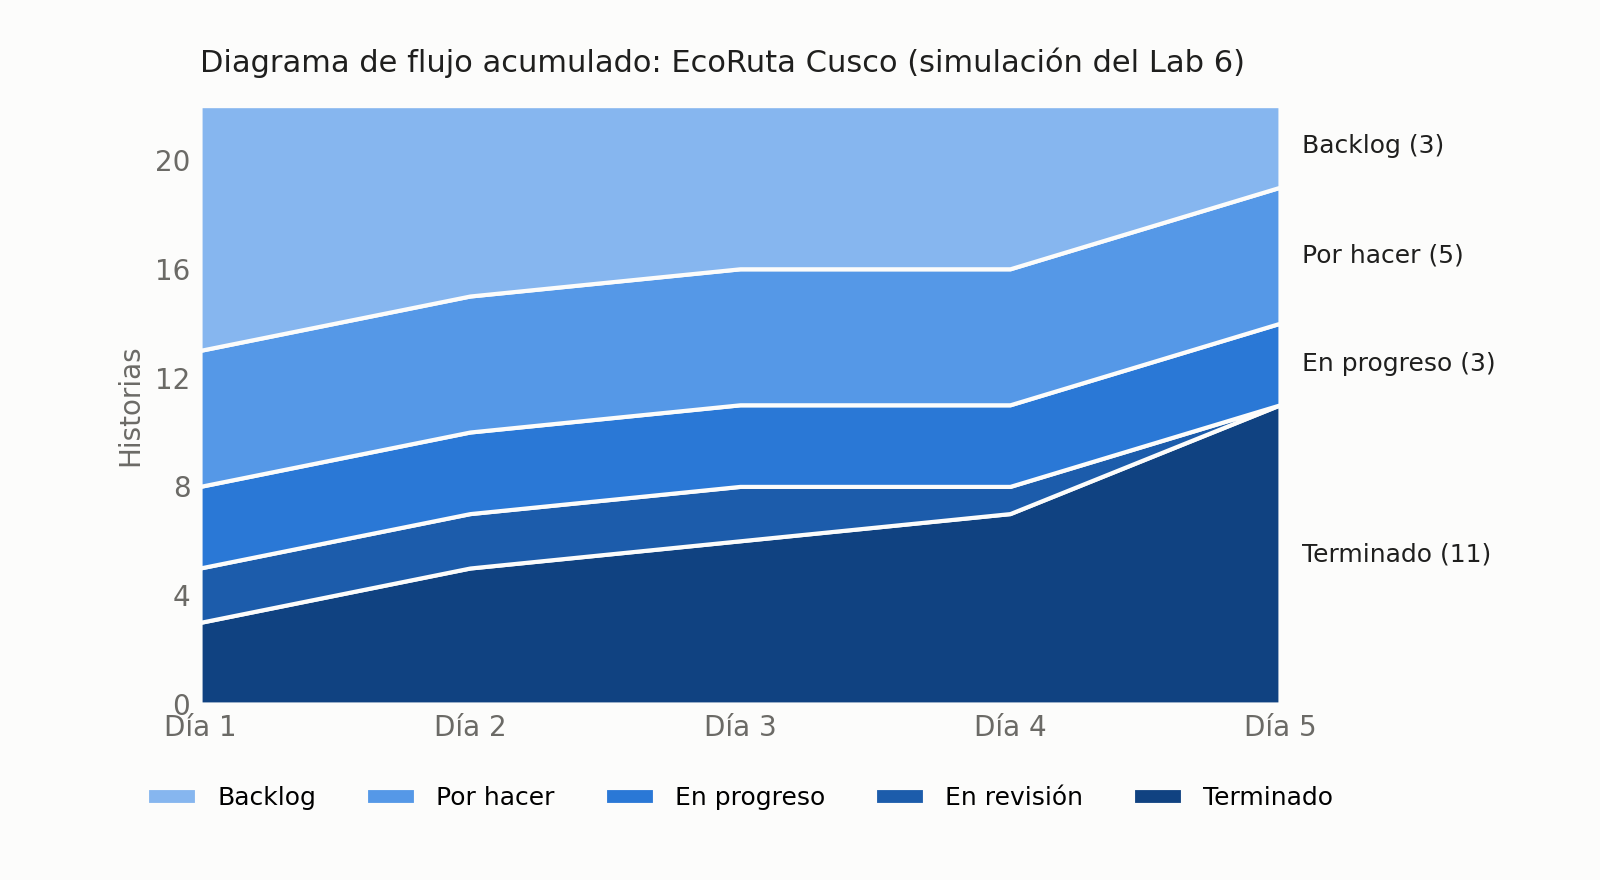
\includegraphics[width=0.9\linewidth]{../img/lab6-flujo-acumulado.png}
  \caption{Diagrama de flujo acumulado de la simulación (22 historias en flujo).}
\end{figure}

Cómo leerlo: el grosor de cada banda es la cantidad de historias en esa columna.
\begin{itemize}
  \item La banda de \textbf{Terminado} crece poco del Día 1 al Día 4 y salta el Día 5: el equipo terminaba lento mientras la revisión estaba atascada.
  \item La banda de \textbf{En revisión} se mantiene llena (2) los Días 1 a 3: ese es el cuello de botella. Se adelgaza cuando el equipo empieza a revisar primero (Días 4 y 5).
  \item \textbf{Por hacer} y \textbf{En progreso} tienen grosor constante (5 y 3) porque los límites WIP las mantienen estables.
\end{itemize}

\subsection{Cuellos de botella detectados}

\begin{center}
\small
\begin{tabularx}{\linewidth}{C{0.5cm} L{2.8cm} Y Y}
\toprule
\textbf{\#} & \textbf{Cuello de botella} & \textbf{Evidencia} & \textbf{Acción tomada} \\
\midrule
1 & \textbf{Revisión} (Días 1 y 3) & En revisión superó su límite (3/2) el Día 1; el Día 3, HU-10 esperó un día completo sin poder pasar a revisión & Regla ``cada día empieza revisando''; quien no tiene trabajo en progreso revisa \\
2 & \textbf{Retrabajo} (Día 4) & HU-03.1 volvió de revisión a En progreso por un criterio no cumplido; su cycle time fue el más alto (5 días) & Trabajo en pareja; revisar los criterios de aceptación \textbf{antes} de programar \\
3 & \textbf{Historias duplicadas} (inicio) & HU-03, HU-08 y HU-09 aparecían junto con sus refinadas & Las originales salieron del flujo (sección 2.2) \\
\bottomrule
\end{tabularx}
\end{center}

% ---------------------------------------------------------------- 5
\section{Entregable}

\subsection{Tablero Kanban activo}

\IfFileExists{../img/lab6-tablero.png}{%
\begin{figure}[H]
  \centering
  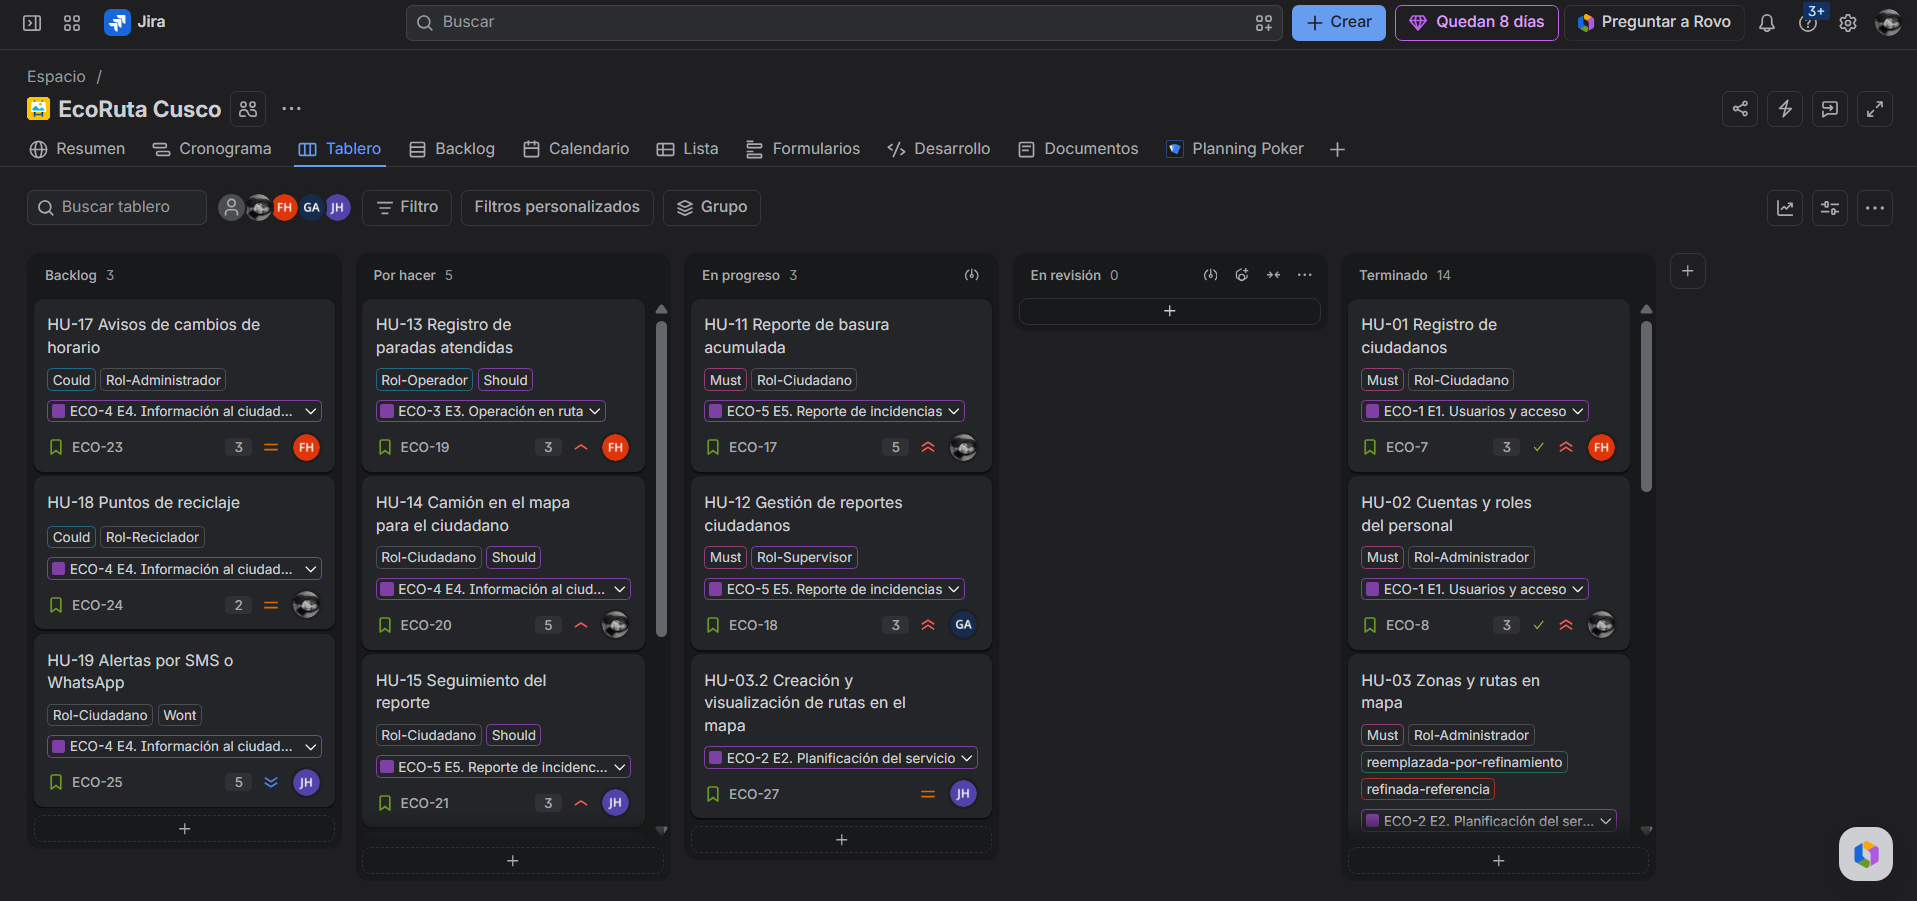
\includegraphics[width=\linewidth]{../img/lab6-tablero.png}
  \caption{Tablero Kanban de EcoRuta Cusco en Jira al cierre del Día 5: Backlog (3), Por hacer (5), En progreso (3), En revisión (0) y Terminado (14, incluidas las 3 historias reemplazadas por refinamiento).}
\end{figure}}{%
\begin{center}\fbox{\parbox{0.9\linewidth}{\centering\vspace{2cm}Captura del tablero Kanban en Jira (\texttt{docs/img/lab6-tablero.png})\vspace{2cm}}}\end{center}}

\subsection{Historias distribuidas correctamente}

Las 22 historias en flujo quedaron así al cierre del Día 5. Cada historia tiene un responsable, y ninguna columna supera su límite:

\begin{center}
\small
\begin{tabular}{L{3cm} C{2cm} C{2.4cm} C{2cm}}
\toprule
\textbf{Columna} & \textbf{Historias} & \textbf{Límite WIP} & \textbf{¿Cumple?} \\
\midrule
Backlog & 3 & --- & \si \\
Por hacer & 5 & 5 & \si \\
En progreso & 3 & 3 & \si \\
En revisión & 0 & 2 & \si \\
Terminado & 11 & --- & \si \\
\bottomrule
\end{tabular}
\end{center}

% ---------------------------------------------------------------- 6
\section{Trabajo extra: tablero actualizado durante la semana}

\begin{itemize}
  \item El tablero se actualizó \textbf{cada día de la simulación} (secciones 3 y 4). Quedó registro en Jira, con un comentario por movimiento, y en el diagrama de flujo acumulado.
  \item Después de la entrega, el tablero queda \textbf{activo} con trabajo en En progreso y Por hacer. El equipo lo seguirá actualizando con el mismo procedimiento: revisar primero, respetar los límites WIP y reponer Por hacer desde Backlog una vez por semana.
\end{itemize}

% ---------------------------------------------------------------- 7
\section{Conclusiones}

\begin{enumerate}
  \item \textbf{Los límites WIP hacen visibles los problemas.} Sin límites, las historias del Día 1 se habrían seguido acumulando en revisión sin que nadie lo notara. Con el límite, el tablero mostró el atasco de inmediato.
  \item \textbf{El cuello de botella del equipo es la revisión, no el desarrollo.} Apareció dos veces (Días 1 y 3). La solución fue un cambio de hábito (``revisar antes de empezar'') y no subir el límite.
  \item \textbf{Terminar es más valioso que empezar.} El Día 5, con la revisión al día, el equipo terminó 4 historias, tantas como en los cuatro días anteriores juntos.
  \item \textbf{Los criterios de aceptación evitan retrabajo.} La única historia devuelta (HU-03.1) falló un criterio que ya estaba escrito desde el Lab 3. Revisarlos antes de programar habría ahorrado 2 días.
  \item \textbf{Las métricas son coherentes entre sí.} Con un cycle time promedio de 2,8 días, un lead time de 4 días y un throughput de 1,8 historias por día, la Ley de Little da un resultado cercano. Estos valores sirven como referencia para prever cuándo se terminarán las historias pendientes.
\end{enumerate}

\end{document}
